\documentclass[12pt,letterpaper,oneside,reqno]{amsart}
\usepackage{amsfonts}
\usepackage{amsmath}
\usepackage{amssymb}
\usepackage{amsthm}
\usepackage{float}
\usepackage{mathrsfs}
\usepackage{colonequals}
\usepackage[font=small,labelfont=bf]{caption}
\usepackage[left=1in,right=1in,bottom=1in,top=1in]{geometry}
\usepackage[pdfpagelabels,hyperindex,colorlinks=true,linkcolor=blue,urlcolor=magenta,citecolor=green]{hyperref}
\usepackage{graphicx}
\usepackage{spverbatim}
\linespread{1.7}
\emergencystretch=1em
\emergencystretch=1em
\usepackage{etoolbox}
\apptocmd{\sloppy}{\hbadness 10000\relax}{}{}
\raggedbottom

\newtheorem{thm}{Theorem}[section]
\newtheorem{cor}[thm]{Corollary}
\newtheorem{lem}[thm]{Lemma}
\newtheorem{examp}[thm]{Example}
\newtheorem{conj}[thm]{Conjecture}
\newtheorem{defn}[thm]{Definition}

\numberwithin{equation}{section}

\title[Secure OIDC implementation using Azure AD and ASP .NET Core]
{Secure OpenID Connect implementation using Azure Active Directory and ASP .NET Core}
\author[Petro Kolosov]{Petro Kolosov}
\author[Dmitrij Kudryashov]{Dmitrij Kudryashov}
\email{kolosovp94@gmail.com}
\urladdr{https://kolosovpetro.github.io}
\email{kudryashov.kd@gmail.com}
\keywords{
    OpenID Connect,
    OIDC,
    Azure Active Directory,
    PKCE,
    OAuth 2.0,
    XSS,
    CSRF,
    ASP .NET Core
}
\date{\today}
\hypersetup{
    pdftitle={Secure OpenID Connect implementation using Azure Active Directory and ASP .NET Framework},
    pdfsubject={
        OpenID Connect,
        OIDC,
        Azure Active Directory,
        PKCE,
        OAuth 2.0,
        XSS,
        CSRF,
        ASP .NET Core,
        Authentication,
        Authorization,
        Azure AD,
        Microsoft Azure,
        Computer security
    },
    pdfauthor={Petro Kolosov},
    pdfkeywords={
        OpenID Connect,
        OIDC,
        Azure Active Directory,
        PKCE,
        OAuth 2.0,
        XSS,
        CSRF,
        ASP .NET Core,
        Authentication,
        Authorization,
        Azure AD,
        Microsoft Azure,
        Computer security
    }
}
\begin{document}
    \begin{abstract}
        Lorem ipsum – псевдо-латинский текст, который используется для веб дизайна, типографии, оборудования,
и распечатки вместо английского текста для того, чтобы сделать ударение не на содержание,
а на элементы дизайна.
    \end{abstract}

    \maketitle

    \tableofcontents


    \section{Definitions}\label{sec:definitions}
    \begin{itemize}
    \item \textbf{Токен доступа (Access Token)} - Это данные, используемые для авторизации на защищенном ресурсе.
    Чаще всего токен доступа в JWT-формате, то есть в виде нескольких последовательных частей,
    разделенных точками.
    Каждая часть содержит base64url-закодированное значение.
    \item \textbf{Токен обновления (Refresh Token)} - Это данные, используемые для получения новых токенов доступа, когда когда текущий токен
    доступа становится недействительным или истекает срок его действия.
    Токены обновления выдаются клиенту сервером авторизации.
    \item \textbf{Владелец ресурса (Resource Owner)} - Субъект, способный предъявить авторизацию для доступа к защищенному ресурсу.
    Когда владельцем ресурса является человек, его называют конечный пользователь.
    \item \textbf{Сервер ресурсов (Resource Server)} - Сервер, который хранит защищенные ресурсы и может обрабатывать запросы к этим ресурсам только
    после проверки наличия соответствующего токена доступа.
    \item \textbf{Клиент (Client)} - Приложение, выполняющее запросы к защищенным ресурсам.
    \item \textbf{Сервер авторизации (Authorization Server)} - Сервер, выдающий токены доступа клиенту после успешной аутентификации.
\end{itemize}


    \section{Statement of the problem}\label{sec:statement-of-the-problem}
    В данной статье мы рассматриваем проблему безопасного хранения и передачи токена доступа между микросервисами.
Разделяют два способа хранения токена доступа, а именно хранение в Local Storage и хранение в файлах cookie.
Local Storage - это механизм веб-браузера, который позволяет веб-приложениям хранить данные локально
на устройстве пользователя.
Важно отметить, что локальное хранилище уязвимо для атак типа Cross-Site Scripting~\cite{spett2005cross}.
Cross-Site Scripting - это тип атаки, суть которого в том чтобы внедрить вредоносный JavaScript код
в выдаваемую html-страницу с целью похищения данных пользователя, например токена доступа.

Различают несколько видов XSS атак:
\begin{itemize}
    \item \textbf{Отражённый XSS (Reflected XSS)} - это тип атаки, при которой вредоносный
    скрипт передается веб-серверу через параметры URL или формы, а затем возвращается обратно в html-код страницы
    без должной фильтрации или экранирования.
    Если пользователь открывает страницу, то скрипт выполняется в браузере, что может привести к потере чувствительных данных,
    например токена доступа.
    \item \textbf{Хранимая XSS (Stored XSS)} - это тип атаки при которой вредоносный скрипт сохраняется на сервере, например
    в базе данных и отображается на веб-страницах.
    Скрипт выполняется в браузерах пользователей, запрашивающих страницы с вредоносным кодом.
    \item \textbf{XSS в DOM-модели} - это тип атаки, при вредоносный скрипт модифицирует DOM-дерево веб-страницы,
    выполняясь в браузере пользователя.
    В большинстве случаев, основан на модификации URL-строки.
\end{itemize}

Другой способ хранить данные это хранить в файлах cookie.
Файлы Cookie - это небольшой фрагмент данных, отправленный веб-сервером и хранимый на устройстве пользователя.
Хранение токенов доступа в файлах Cookie невелирует потенциальные XSS атаки, так как достаточно установить флаг HttpOnly,
запрещающий JavaScript коду чтение данных из файлов Cookie.
Передача токенов доступа в запросах осуществляется с использованием JavaScript Http методов
с флагом \texttt{\{ withCredentials: true \}},
таким образом, если файлы cookie существуют, то они передается вместе с запросом, но все еще не могут быть прочитаны используя
JavaScript.
Пример такого запроса следующий
\begin{spverbatim}
    return this.httpClient.post<TokensResponse>(
        this.baseUrl + this.sessionsRoute,
        command,
        { withCredentials: true });
\end{spverbatim}

Однако, файлы cookie уязвимы для Cross-Site Request Forgery (CSRF) атак~\cite{siddiqui2011cross}.
Cross-Site Request Forgery (CSRF) - представляет собой атаку при которой злоумышленник создает переадресацию
на ресурс, где пользователь имеет активную сессию.
Основной принцип Cross-Site Request Forgery (CSRF) проилюстрирован ниже

\begin{figure}[H]
    \centering
    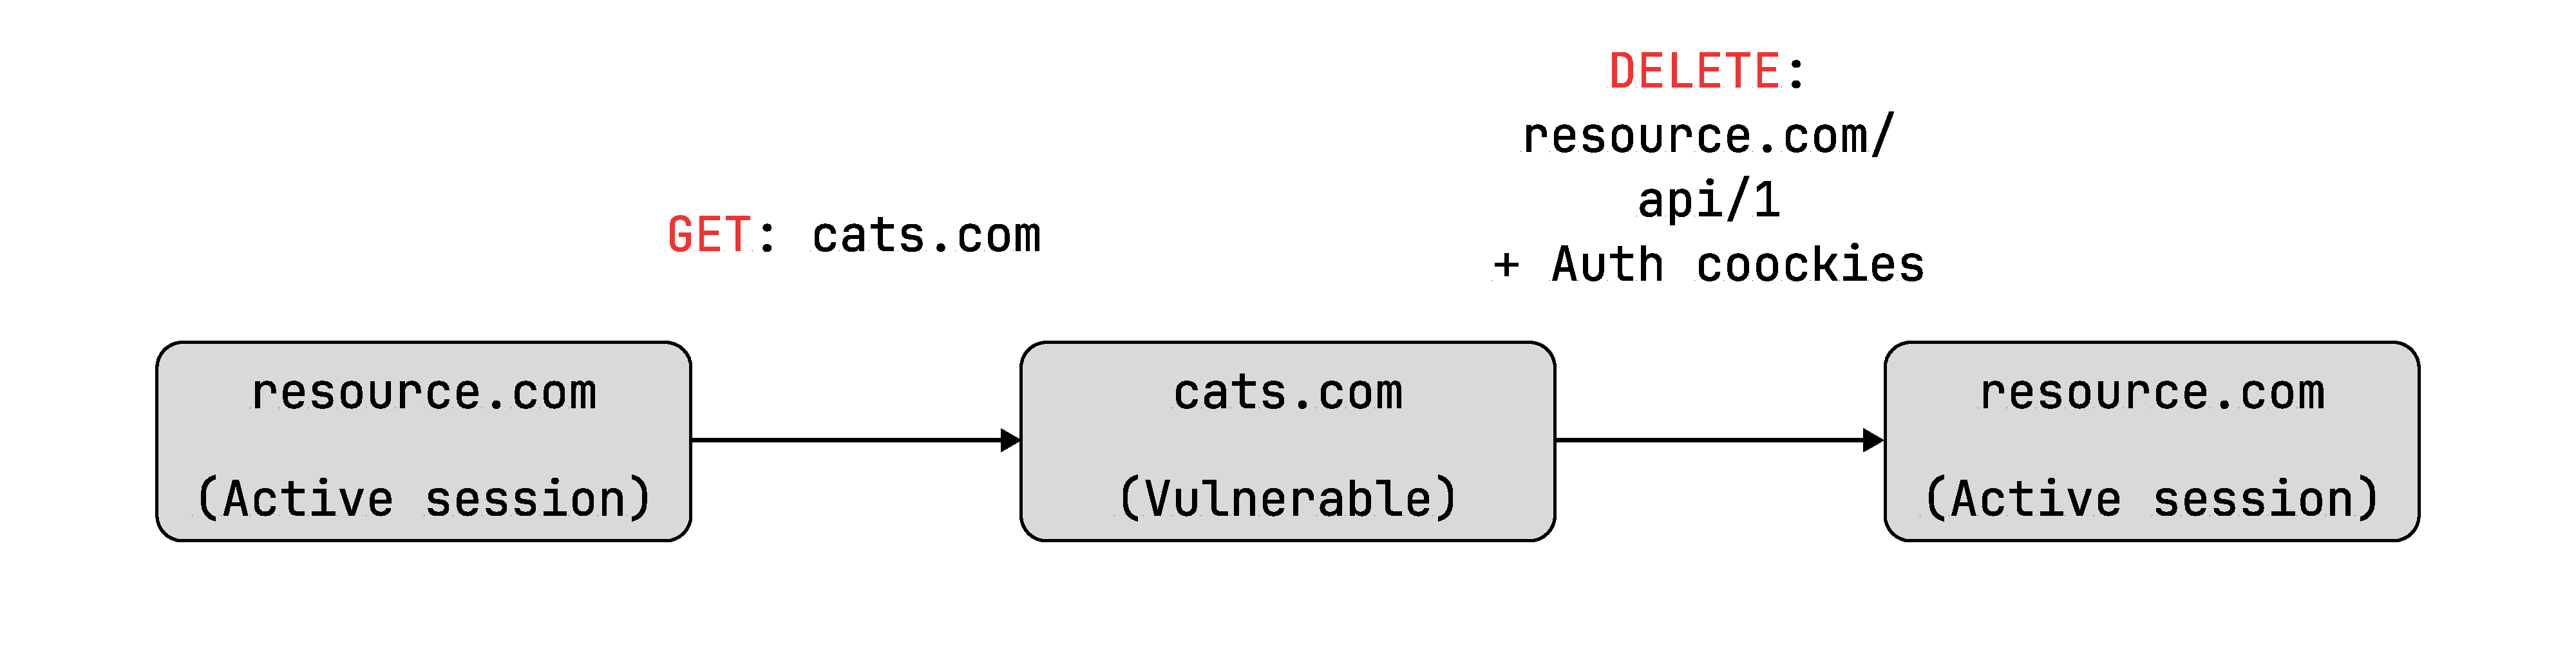
\includegraphics[width=1\textwidth]{img/Csrf_diagram}
    ~\caption{CSRF attack principle diagram.}\label{fig:csrf_diagram}
\end{figure}

Файлы cookie имеют параметр \texttt{SameSite}, который определяет будут ли они отправлены вместе с запросом на сайт,
имеющим другой домен.

Существует три возможных значения параметра \texttt{SameSite}:

\begin{itemize}
    \item \textbf{None} - прямо указывает, что на передачу cookie-файлов не накладывается никаких ограничений.
    \item \textbf{Lax} - разрешает передачу cookie только безопасными HTTP-методами, которыми, согласно
    RFC 7231~\cite{fielding2014rfc}, являются \texttt{GET, HEAD, OPTIONS} и \texttt{TRACE}.
    \item \textbf{Strict} - является самым строгим вариантом безопасности и блокирует отправку cookie с любыми
    запросами на сайт под другим доменом.
    Файлы cookie будут передаваться только в пределах того домена, с которого они и были установлены.
\end{itemize}

Таким образом, значения параметра \texttt{SameSite} такие как \texttt{Lax} и \texttt{Strict} защищают пользователя
от CSRF-атаки, так как блокируют прикрепление файлов cookie к запросу, что был инициирован ресурсом злоумышленника.

Другие методы защиты от CSRF описаны в~\cite{owaspCsrf}.


    \section{Introduction to OpenID Connect}\label{sec:introduction-to-open-id-connect}
    OpenId Connect — это дополнительный уровень~\cite{siriwardenaOpenid2020, sakimuraOpenid2014} идентификации поверх
протокола~\cite{hardt2012oauth} OAuth 2.0.
Он позволяет клиентам проверять личность конечного пользователя на основе аутентификации,
а также получать базовую информацию о профиле конечного пользователя.

OAuth 2.0 — это протокол, позволяющий стороннему приложению получить ограниченный доступ к HTTP-сервису, либо от имени
владельца ресурса, организуя взаимодействие по утверждению между владельцем ресурса и HTTP-сервисом, либо путем разрешения
стороннему приложению получить доступ от своего имени.

В традиционной модели аутентификации клиент-сервер, клиент запрашивает ресурс с ограниченным доступом
через аутентификацию с использованием пары логин-пароль.
Для того чтобы предоставить стороннему приложению доступ к ресурсам,
владелец ресурса (пользователь) делится своими учетными данными (логином и паролем) со сторонним приложением.
Этот подход создает ряд проблем и ограничений~\cite{hardt2012oauth}:
\begin{itemize}
    \item Сторонние приложения должны хранить учетные данные (логин и пароль) владельца ресурса для дальнейшего использования,
    бывает так, что пароль хранится в явном виде в базе данных.
    \item Сторонние приложения обязаны поддерживать аутентификацию с помощью пароля, несмотря на недостатки безопасности,
    присущие паролям.
    \item Сторонние приложения получают полный доступ к защищенным ресурсам владельца ресурса (пользователя),
    оставляя владельцев ресурсов без какой-либо возможности ограничить продолжительность доступа или подмножество
    доступных ресурсов (scope).
    \item Владельцы ресурсов (пользователи) не могут отозвать доступ к отдельному третьему лицу без отзыва доступа для всех
    третьих лиц, и должны отозвать доступ только путем изменения пароля.
    \item Взлом либо утечка данных из любого стороннего приложения приводит к потере пароля конечного пользователя и
    всех данных, защищенных этим паролем.
\end{itemize}

OAuth 2.0 решает эти проблемы путем введения уровня авторизации и разделения роли клиента (сервис авторизации) и
владельца ресурса (пользователя).
В OAuth 2.0 клиент запрашивает доступ к ресурсам, контролируемым владельцем ресурса и размещенным на сервере ресурса.
Вместо того чтобы использовать учетные данные владельца ресурса для доступа к защищенным ресурсам, клиент получает токен доступа.

OAuth 2.0 with the Proof of Key Code Exchange~\cite{bradley2015rfc} flow показан ниже
\begin{figure}[H]
    \centering
    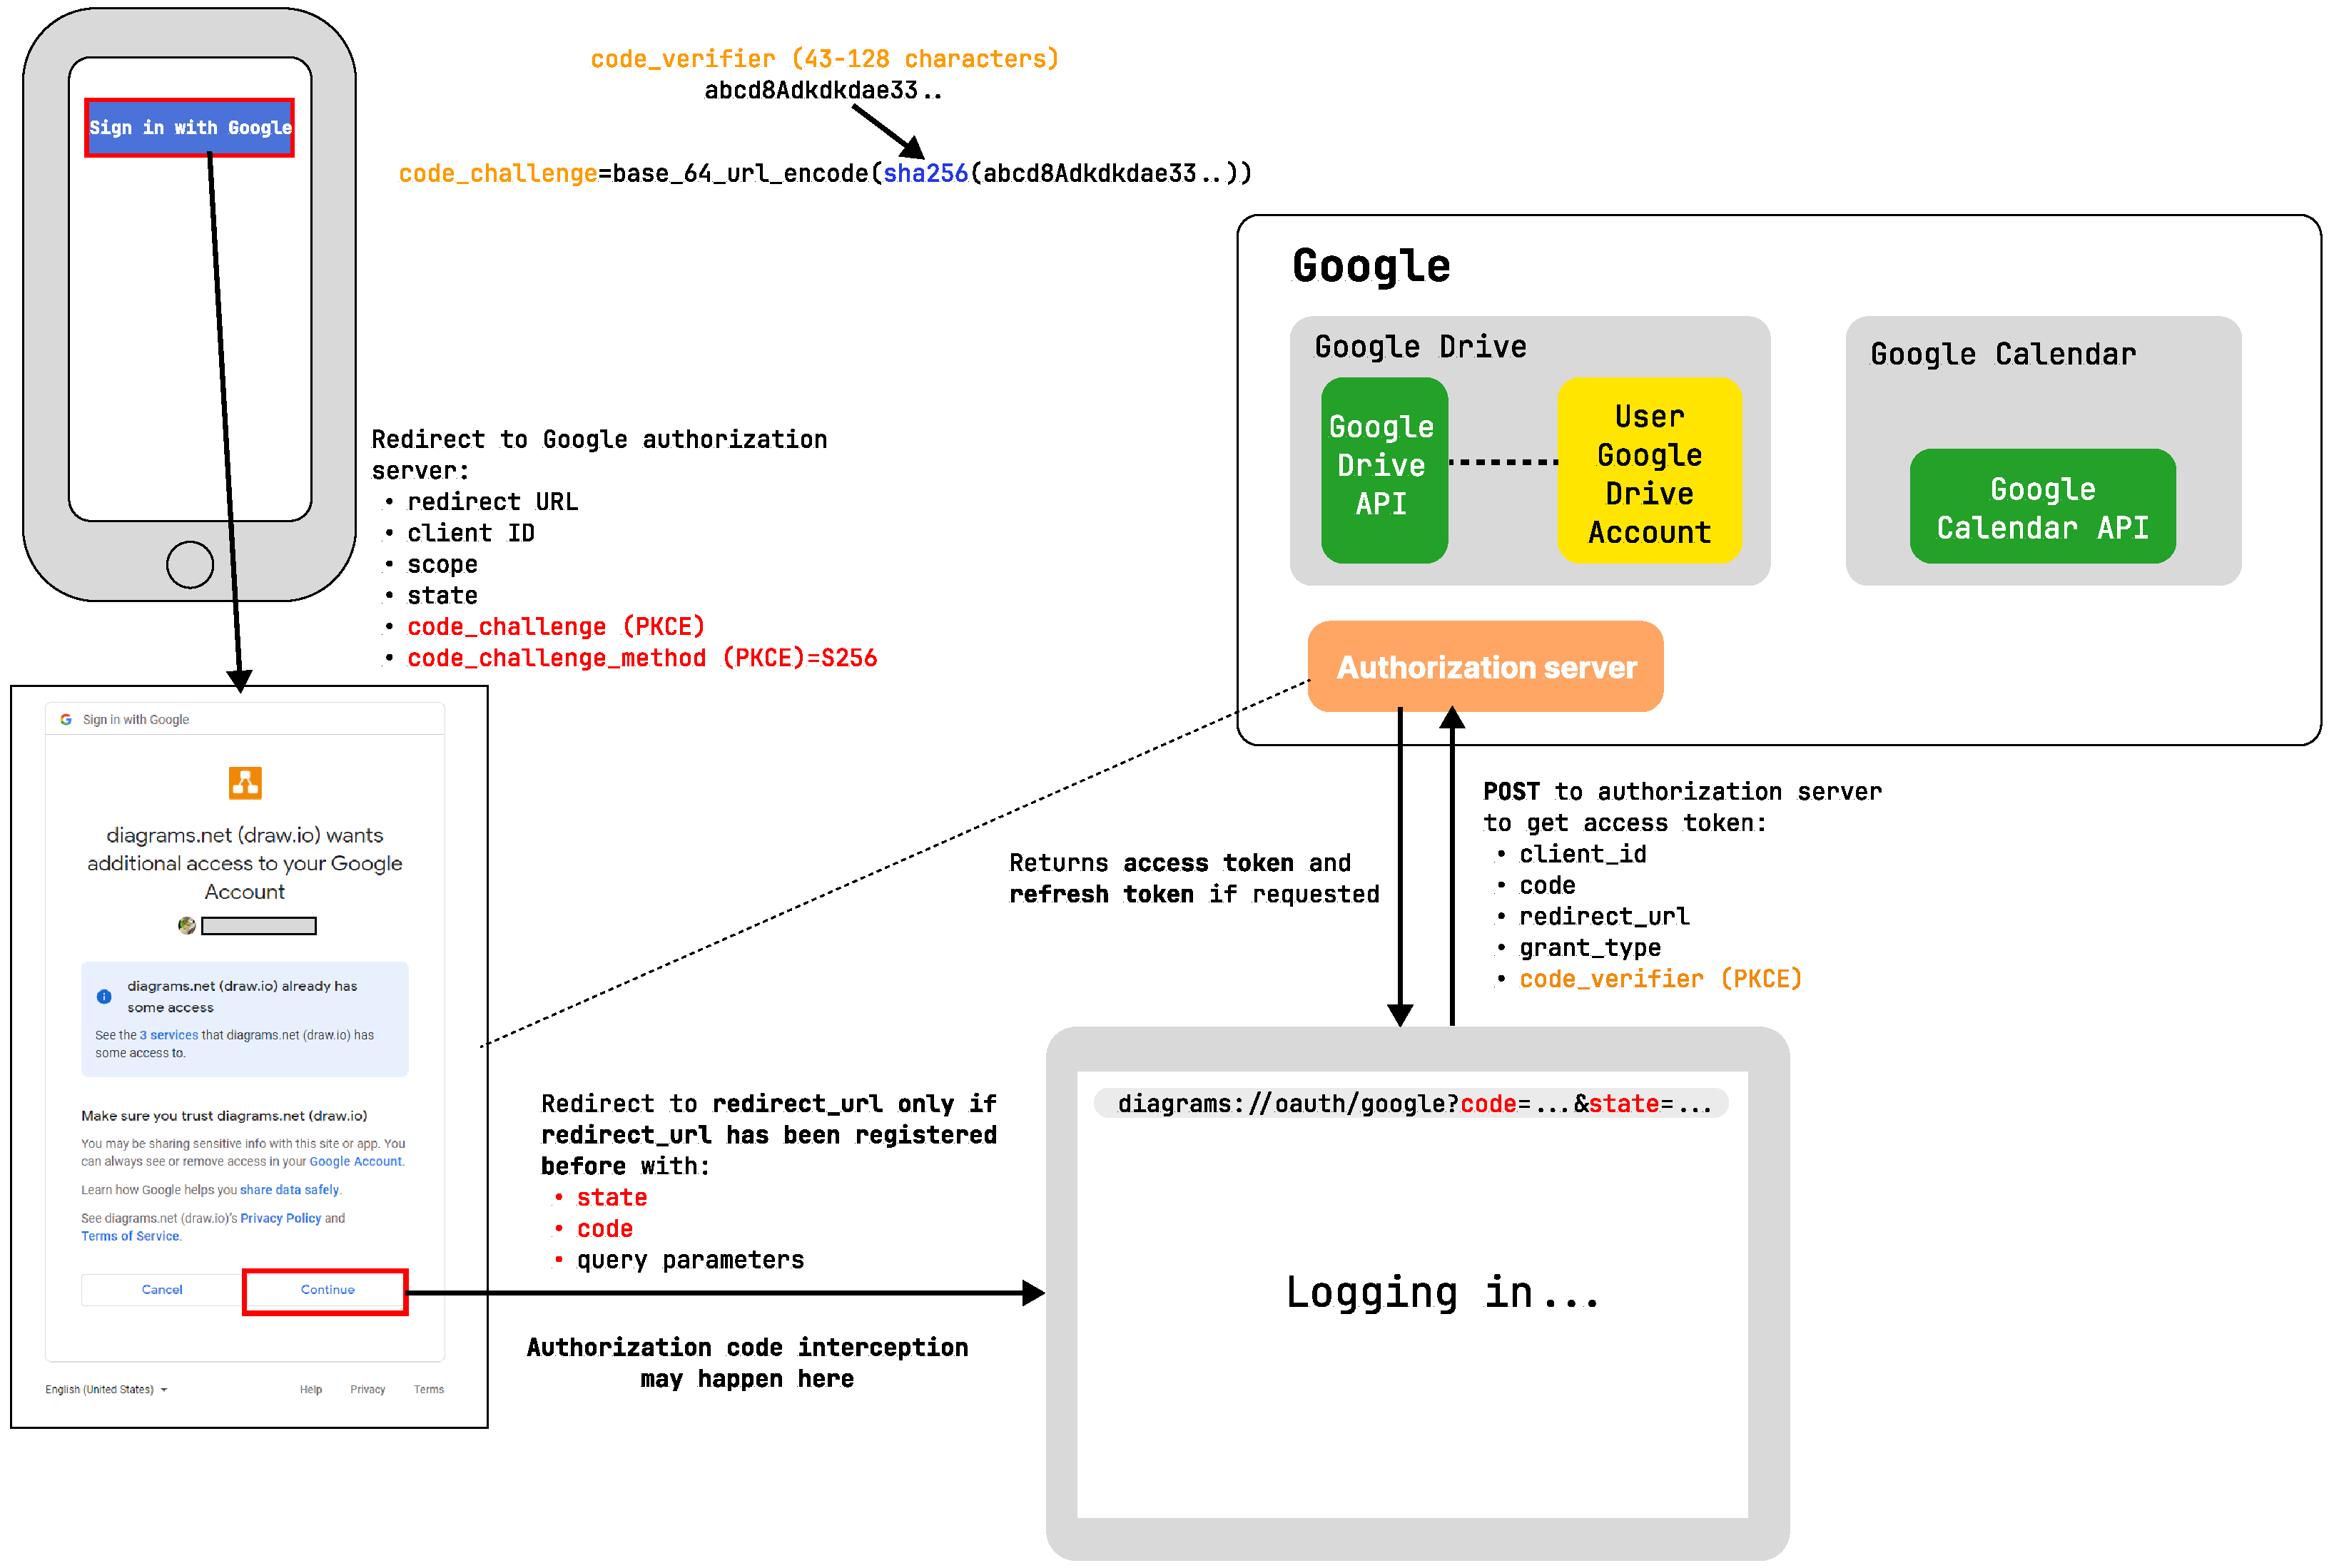
\includegraphics[width=1\textwidth]{img/OAuthPkceScheme_1570_1055}
    ~\caption{OAuth 2.0 with PKCE flow diagram.}\label{fig:figure2}
\end{figure}

\begin{enumerate}
    \item После нажатия на кнопку \texttt{Sign in with Google} происходит перенаправление на ендпоинт авторизации,
    на котором владелец ресурса должен ввести свои учетные данные, а так же согласиться с некоторыми условиями.
    Особое внимание стоит обратить на code\_challenge и code\_challenge\_method, первое представляет собой некоторую строку,
    которая будет закодирована с помощью метода кодировки указанного в параметре запроса code\_challenge\_method.
    В дальнейшем, при обмене полученного кода на токен доступа и обновления, мы должны будем предъявить значение code\_verifier,
    которое равно ранее закондированному code\_challenge.
    \item После успешной аутентификации, произойдет перенаправление на адресс \texttt{redirect\_uri}.
    \item После получения авторизационного кода происходит обмен этого кода на токены доступа (access token) и
    обновления (refresh token).
    Если ранее, при переадресации владельца ресурса на авторизационный ендпоинт, мы указывали \texttt{code\_challenge}
    и \texttt{code\_challenge\_method},
    то теперь, при обмене кода на токены, мы обязаны передать в запросе значение \texttt{code\_verifier}.
\end{enumerate}
Здесь мы упоминаем такие определения, как code и state.
\begin{itemize}
    \item \textbf{Code} - это код авторизации, который получается с помощью сервера авторизации и является посредником
    между клиентов и владельцем ресурса.
    Перед тем как сервер авторизации перенаправит владельца ресурса обратно на клиент, сервер авторизации проверяет
    подлинность владельца ресурса.
    Так образом поскольку владелец ресурса аутентифицируется только на сервере авторизации, его учетные данные никогда
    не передадутся клиенту.
    \item \textbf{State} - значение, используемое клиентом для сохранения состояния между запросом на авторизацию и
    обратным вызовом (callback).
    Сервер авторизации включает это значение при перенаправлении агента пользователя обратно клиенту.
    Этот параметр используется для предотвращения Cross-Site Request Forgery (CSRF) атак.
\end{itemize}

Authorization code flow with PKCE является протоколом, который представляет секрет, созданный клиентом,
который может быть проверен сервером авторизации.
Этот секрет называется \texttt{code\_verifier}.
Клиент хеширует значение \texttt{code\_verifier} и записывает его в параметр \texttt{code\_challenge}.
PKCE решает проблему безопасного обмена кода.
Если злоумышленнику удастся заполучить авторизационный код, то у него не получится обменять
его на токены доступа и обновления.
Таким образом, мы гарантируем тот факт, что обмен кода на токены производит то же самое приложение, что и выполняло
аутентификацию.
В некотором роде, PKCE можно сравнить с цифровой подписью процесса аутентификации.
При обмене кода авторизации на токены обязательно нужно указать \texttt{code\_verifier}.


    \section{Authentication flow}\label{sec:authentication-flow}
    Рассмотрим более практичный подход, учитывающий все рассмотренные ранее аспекты.
Применяя современные фреймворки, такие как ASP.NET Core и Angular, можно реализовать следующий флоу аутентификации
в соответствии с приведенной ниже схемой
\begin{figure}[H]
    \centering
    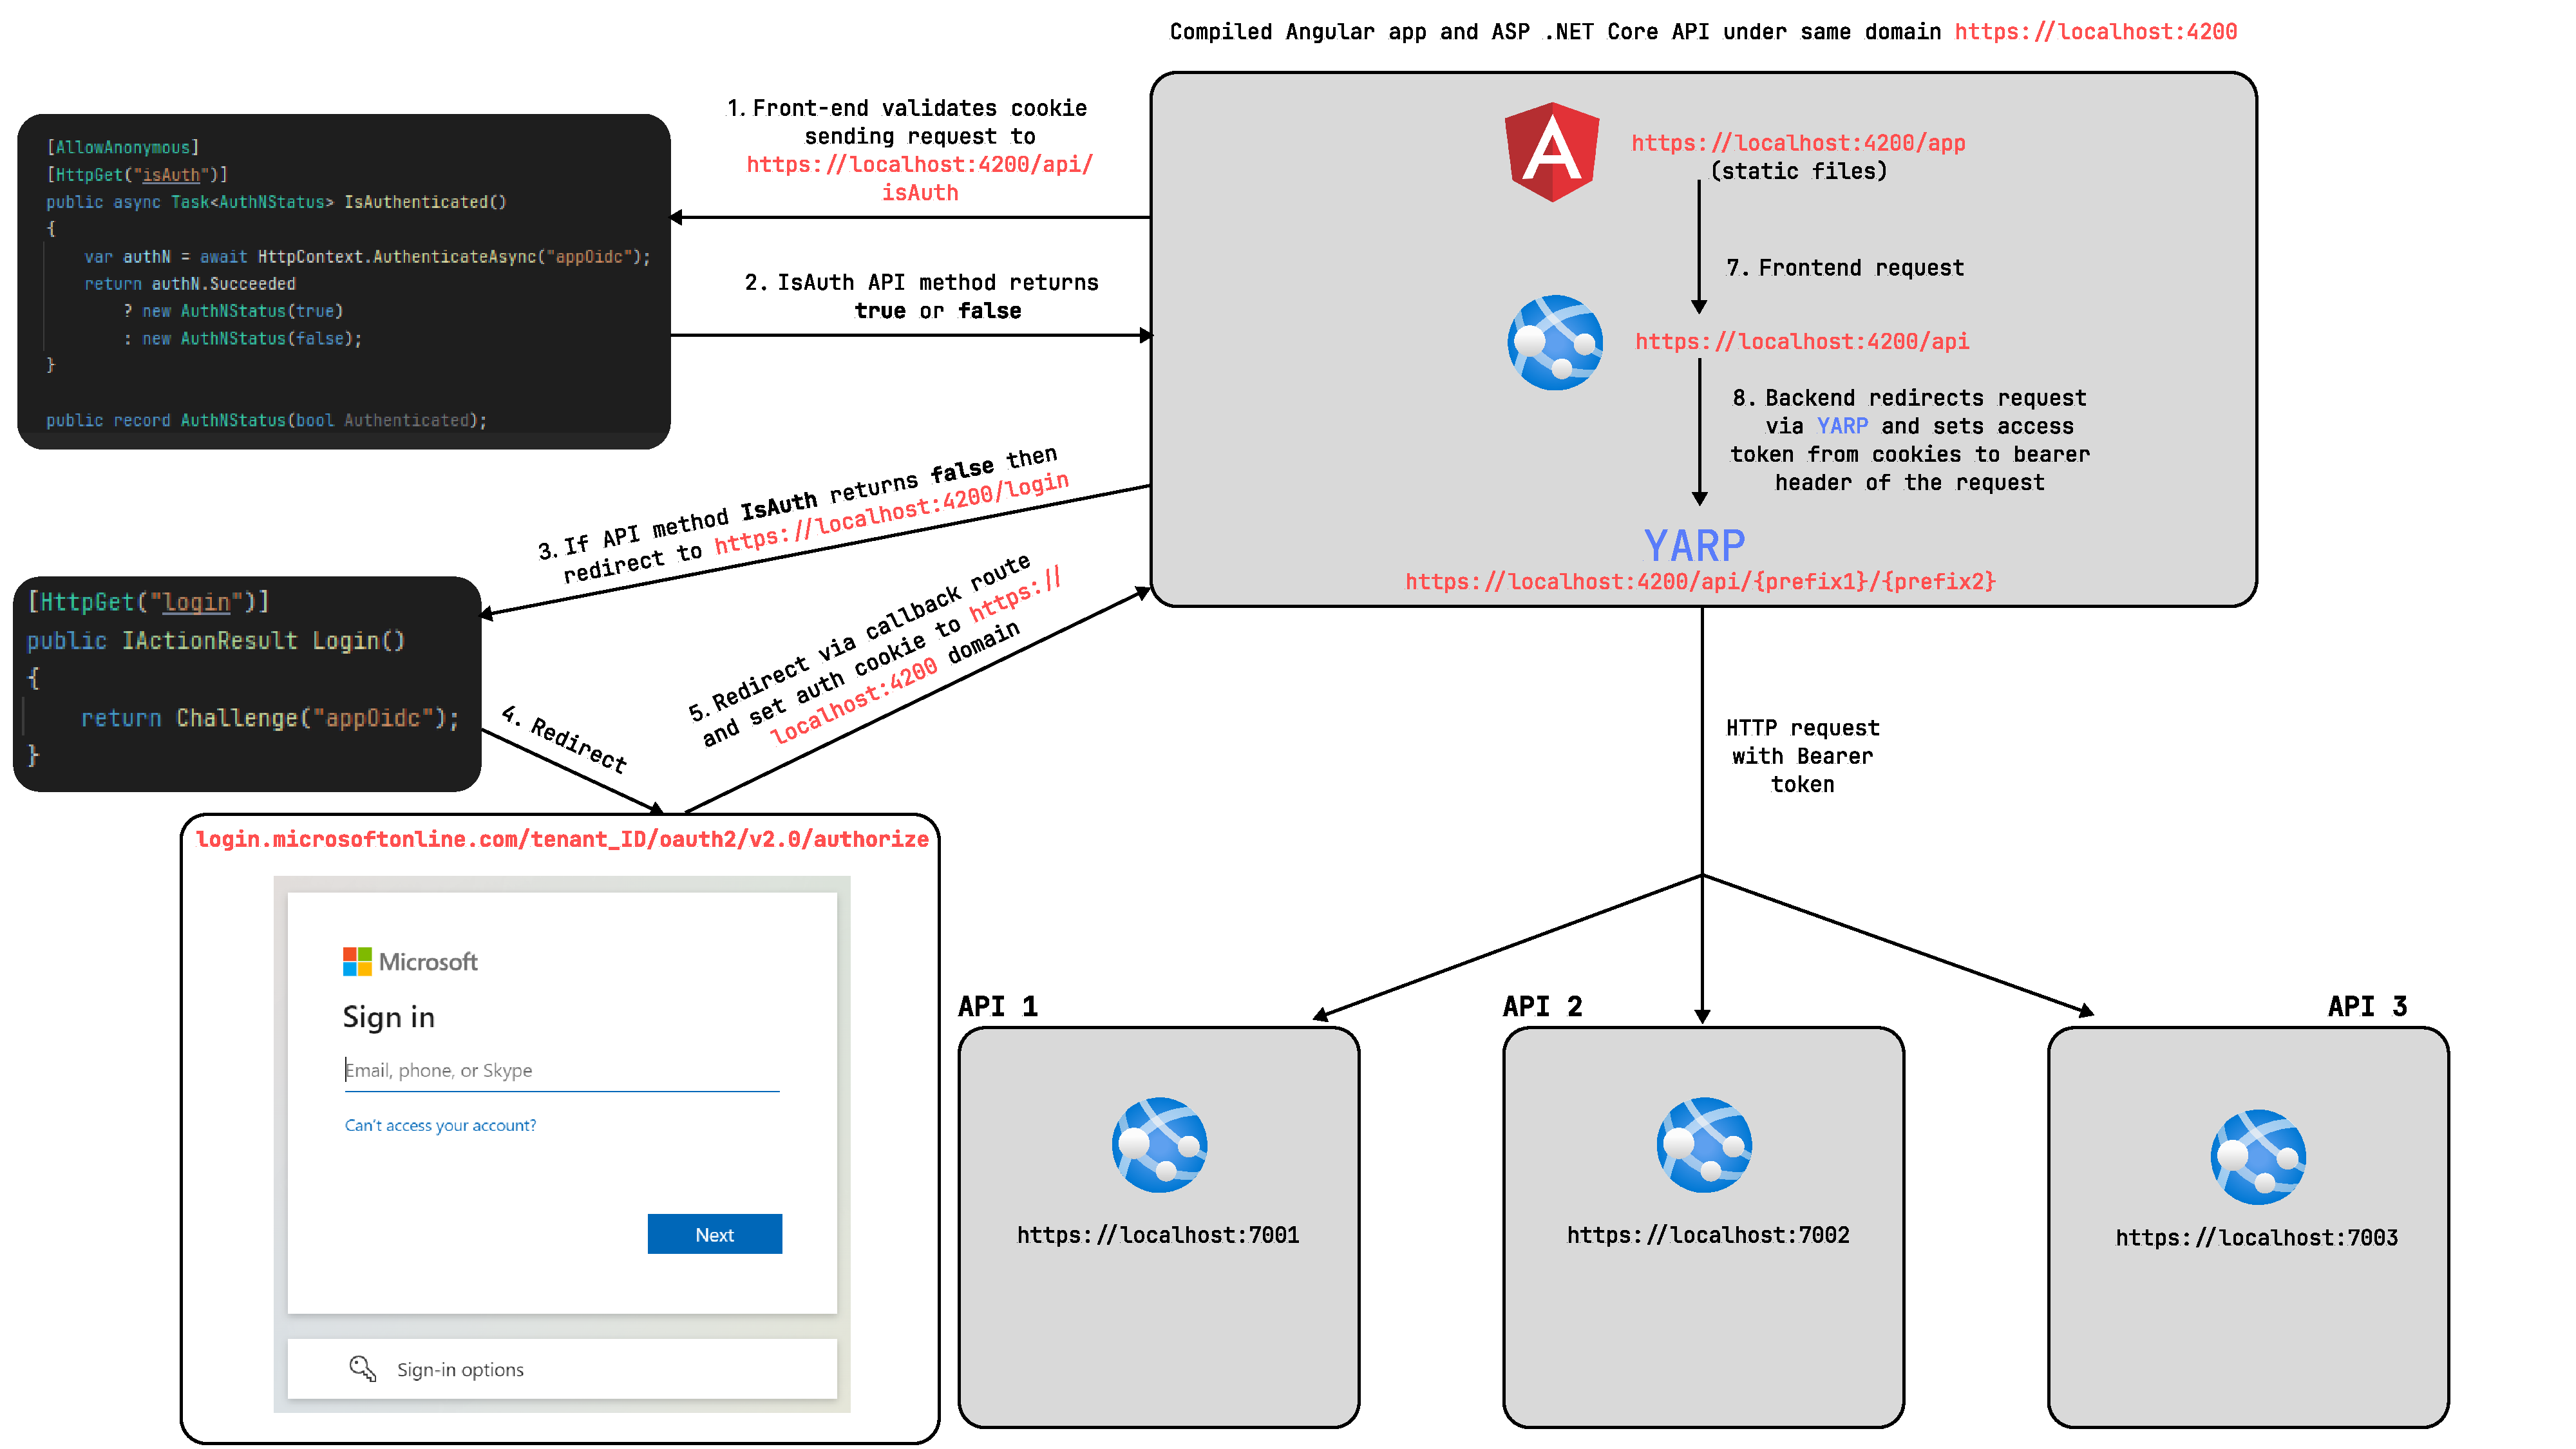
\includegraphics[width=1\textwidth]{img/Auth_flow_updated}
    ~\caption{Authentication flow diagram.}\label{fig:figure}
\end{figure}

Таким образом, весь процесс аутентификации можно описать в виде восьми этапов, таких как
\begin{enumerate}
    \item Скомпилированное Angular-приложение отправляет запрос к ендпоинту ASP.NET Core API для проверки текущего
    состояния аутентификации.
    Angular-приложение представляет собой набор предварительно скомпилированных пакетов, которые раздаются через
    тот же ASP.NET Core API на ендпоинте \texttt{/app}, что позволяет отказаться от кросс-доменных запросов и
    надежно хранить токены в файлах cookie.
    \item Ендпоинт ASP.NET Core API отвечает либо со HTTP статус кодом \texttt{200 (OK)} или \texttt{401 (Unauthorized)}
    \item Если на предыдущем шаге получен статусный код \texttt{401 (Unauthorized)}, то браузер перенаправляется
    на ендпоинт \texttt{/login} API ASP.NET Core, в ином случае пользователь получает доступ к защищенным ресурсам
    \item Метод Login ASP.NET Core приложения перенаправляет браузер на сайт авторизации
    Azure AD \texttt{login.microsoftonline.com/tenant/oauth2/v2.0/authorize}, где пользователь вводит свои учетные данные.
    Важно уточнить, что для получения ID-токена нам необходимо поместить параметр \texttt{openid} в область видимости (scope)
    \begin{spverbatim}
    serviceCollection
    .AddAuthentication(options => {...})
    .AddCookie(CookieAuthenticationDefaults.AuthScheme,
        options => {...})
    .AddOpenIdConnect(AuthConstants.AppOidc, options =>
    {
        ...
        options.Scope.Add("openid");
    });
\end{spverbatim}
    \item После успешной аутентификации на стороне Azure AD, браузер перенаправляется уже с установленными
    файлами cookie на \texttt{callback\_url}, который определен при регистрации приложения в Azure AD\@.
    В этот момент в флоу включается \texttt{TickerStore}~\cite{microsoftIticketstore2023, ticketStore_2023},
    который нужен для управления сессиями пользователей.
    Каждая сессия хранится в базе данных как сущность \texttt{UserSessionEntity}.
    \begin{spverbatim}
    public class UserSessionEntity
    {
        public Guid Id { get; set; }
        public DateTimeOffset CreatedAt { get; set; }
        public DateTimeOffset ExpiresAt { get; set; }
        public DateTimeOffset UpdatedAt { get; set; }
        public DateTimeOffset DateOfLastAccess { get; set; }
        public byte[] Value { get; set; }
    }
\end{spverbatim}
    Свойство Value типа \texttt{byte[]} содержит сериализованный \texttt{AuthenticationTicket}~\cite{microsoftAuthenticationTicket2023}
    объект, содержащий всю необходимую информацию, такую как ID-токен,
    токен доступа (access token) и токен обновления (refresh token).
    Класс \texttt{TickerStore} реализует интерфейс \texttt{ITickerStore}, который предлагает 4 метода:
    \texttt{StoreAsync, RenewAsync, RetrieveAsync, RemoveAsync}.
    \begin{itemize}
        \item Метод \texttt{StoreAsync} выполняется сразу после аутентификации на сервере авторизации, он сохраняет
        сессию пользователя в базе данных.
        \item Метод \texttt{RenewAsync} в нашем случае используется фоновым сервисом для обновления пользовательских сессий.
        \item Метод \texttt{RetrieveAsync} выполняется каждый раз, когда запрос отправляется на ендпоинт,
        помеченный \texttt{[Authorize]} атрибутом.
        \item Метод \texttt{RemoveAsync} выполняется по истечении срока действия cookie-файлов, а также используется
        тем же \texttt{RefreshBackgroundService} для удаления сессий, которые не использовались в течение длительного времени.
    \end{itemize}
    Пример реализации \texttt{TicketStore} можно найти на~\cite{ticketStore_2023}.
    Пример инъекции зависимостей (DI) \texttt{TicketStore} можно найти на~\cite{ticketStoreDI_2023}.
    На этом шаге происходит настройка аутентификационных cookie.
    \item Шаг 1 здесь повторяется, но теперь HTTP-запрос обязательно должен быть с кодом состояния \texttt{200 (OK)}.
    \item Скомпилированное фронтенд-приложение Angular отправляет запрос к ASP.NET Core API c cookie-файлами.
    Микросервис, принимающий запрос, используя библиотеку \texttt{YARP}~\cite{microsoftYarp2021}, вынимает из
    cookie файлов токен доступа и кладет его в заголовок, после чего перенаправляет запрос на один из микросервисов.
    Конфигурация \texttt{YARP} осуществляется в соответствии с~\cite{yarpDI_2023,yarpSectionAppSettings_2023}.
    \item Если на предыдущем шаге был получен статусный код \texttt{401 (Unauthorized)}, то шаг 1 повторяется.
\end{enumerate}


    \section{Refresh token flow}\label{sec:refresh-token-flow}
    Реализация обновления токенов пользователя крайне проста.
Нам нужно создать фоновый сервис~\cite{microsoftHostedservice2023}, который будет каждые несколько минут выбирать из
базы данных те сессии, которые скоро истекут,
затем фоновый сервис должен десериализовать объект \texttt{AuthenticationTicket}~\cite{microsoftAuthenticationTicket2023}
у каждой найденой сессии, из десериализованного объекта
сервис возьмет токен обновления и отправит запрос на сервер авторизации с целью получения новых токенов доступа,
обновления и ID-токена.
Новые токены заменяют старые в объекте \texttt{AuthenticationTicket}, после чего объект нужно заного сериализовать и
установить уже сериализованный объект в свойство \texttt{Value}.
Кроме того, в ответе сервера авторизации в поле \texttt{ExpiresAt} будет число, которое говорит о том через какое время
(в секундах) истечет токен доступа,
фоновый сервис должен обновить свойство ExpiresAt у объекта \texttt{UserSessionEntity}UserSessionEntity, добавив
к текущему времени секунды, полученные из ответа запроса.

Помимо обновления пользовательских сессий, фоновый сервис отвечает за удалений сессий, которые долго не использовались.
Каждые несколько минут выбираются сессии, их свойства \texttt{DateOfLastAccess} сравнивается с текущем временем,
в случае если разница между двумя датами больше 3 суток - сессия удаляется.
Каждый раз когда пользователь совершает действие на сайте, свойство \texttt{DateOfLastAccess} обновляется.

Реализация фонового сервиса может быть выполнена в соответствии с приведенными
ссылками~\cite{backroundService_2023, configurationBackgroundService_2023}.


    \section{Conclusions}\label{sec:conclusions}
    В данной статье мы рассмотрели проблему безопасного хранения и передачи токенов доступа между микросервисами.
Особое внимание было уделено возможным уязвимостям при передаче токенов доступа, таким как как Cross-Site Scripting (XSS) и Cross-Site Request Forgery (CSRF).

Для устранения данных уязвимостей необходимо хранить авторизационные токены в файлах cookie, с обязательными
настройками \texttt{HttpOnly} и \texttt{SameSite} так что значения \texttt{SameSite} должны быть \texttt{Lax} или \texttt{Strict},
таким образом файлы куки передаются либо на безопасные \texttt{HTTP} методы, либо не передаются вовсе.

Аутентификация должна быть реализована с использованием протокола OIDC~\cite{siriwardenaOpenid2020, sakimuraOpenid2014}, а Authorization code flow с помощью PKCE~\cite{bradley2015rfc}.
олее подробно основной принцип работы протокола OIDC описан в главе 2.

Аутентификация пользователя происходит по протоколу Open ID Connect~\cite{siriwardenaOpenid2020, sakimuraOpenid2014} через Authorization code flow with PKCE~\cite{bradley2015rfc}.
Подробнее принцип работы протокола Open ID Connect и Authorization code flow with PKCE изложен во главе 2.

Так же в работе был предложен механизм аутентификации/авторизации основанный на ASP.NET Web API бекенде и Angular фронтенд приложении
под единым доменом.
Таким образом исключается необходимость передачи авторизационных куки на ресурсы под другими доменами.
Передача токена доступа на микросервисы происходит по средствам Reverse Proxy YARP~\cite{microsoftYarp2021}, таким образом что
токен доступа автоматически подставляется в заголовок запроса.

Кроме того, мы предложили механизм обновления токена доступа через классы \texttt{TicketStore}~\cite{microsoftIticketstore2023} и \texttt{HostedService}~\cite{microsoftHostedservice2023}.
Таким образом, \texttt{TicketStore} проверяет каждый запрос на истечение срока действия токена доступа.
В случае истечения срока действия токена доступа он обновляется с помощью микросервиса авторизации.
Хранилище \texttt{TicketStore} также хранит пары токенов доступа и обновления внутри
\texttt{AuthenticationTicket} entity~\cite{microsoftAuthenticationTicket2023}.

Кроме этого, в работе был предложен механизм обновления токена доступа через реализацию \texttt{TicketStore}~\cite{microsoftIticketstore2023} и \texttt{HostedService}~\cite{microsoftHostedservice2023}.
Таким образом, \texttt{TicketStore} отвечает за проверку каждого запроса на истечение срока действия токена доступа.
В случае истечения срока действия токена доступа, токен доступа обновляется с помощью запроса к эндпоинту сервиса авторизации.
Также задача \texttt{TicketStore} состоит в сохранении токена доступа и токена обновления, которые являются частью \texttt{AuthenticationTicket}~\cite{microsoftAuthenticationTicket2023}.
Hosted Service необходим для фонового обновления истекающих токенов доступа, чтобы поддерживать сессии пользователей активными.

В статье мы решили проблему безопасного хранения токена доступа и передачи его между микросервисами,
а так же предложили решения выявленным уязвимостям вида Cross-Site Scripting (XSS) и Cross-Site Request Forgery (CSRF).

    \bibliographystyle{unsrt}
    \bibliography{SecureAzureOIDC}
    \noindent \textbf{Version:} \texttt{Local-0.1.0}

\end{document}
